\chapter{EIT-based Pressure Sensor Performance Metrics}
\label{appendix-D}

\section{Noise Removal}
\begin{figure*}[h!]
	\centering
	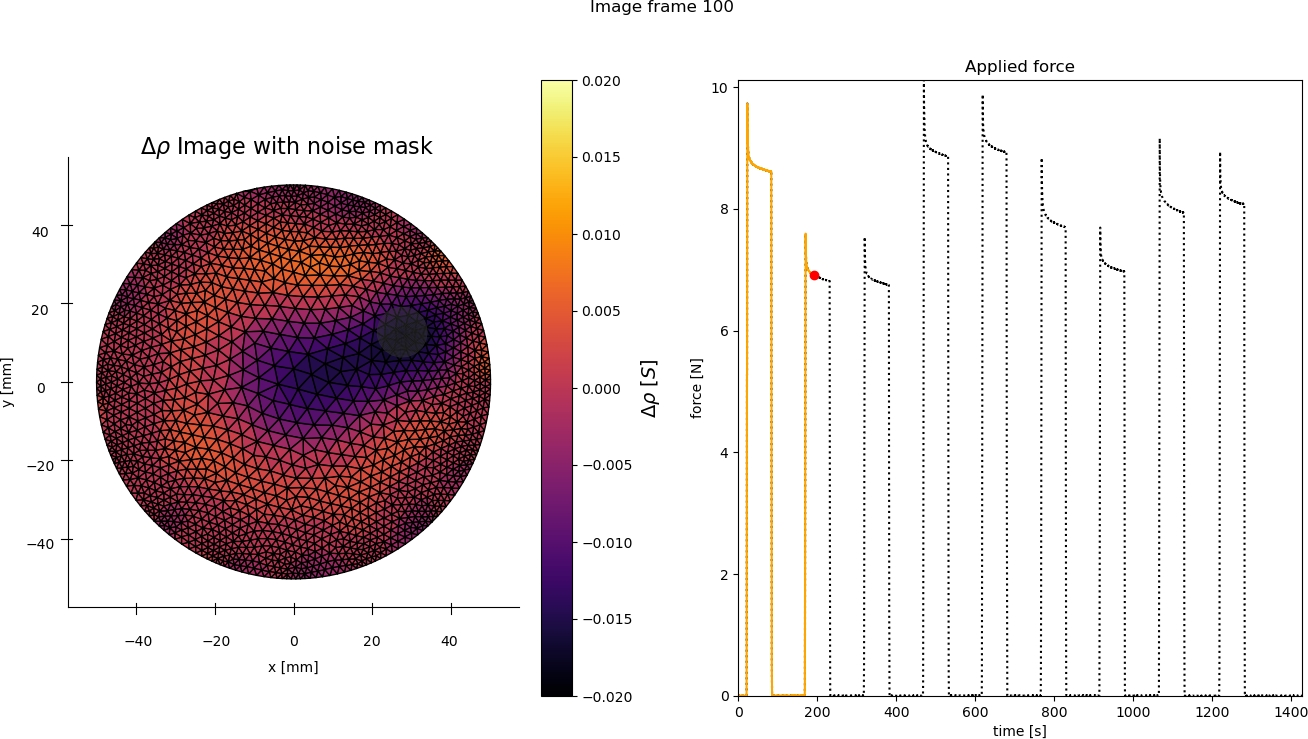
\includegraphics[width=\linewidth]{Figures/CBSR_9p_2_9push_25strain_60s_1mA_4_frame100_noise_mask.jpg}
	\caption{An experimental snapshot. Left: Before executing the performance metrics calculations, the noise floor mask was applied to the 9\% CBSR material. Right: Time series force data}
	\label{fig:noise_floor_mask_9p}
\end{figure*}
\begin{figure}[H]
	\centering
	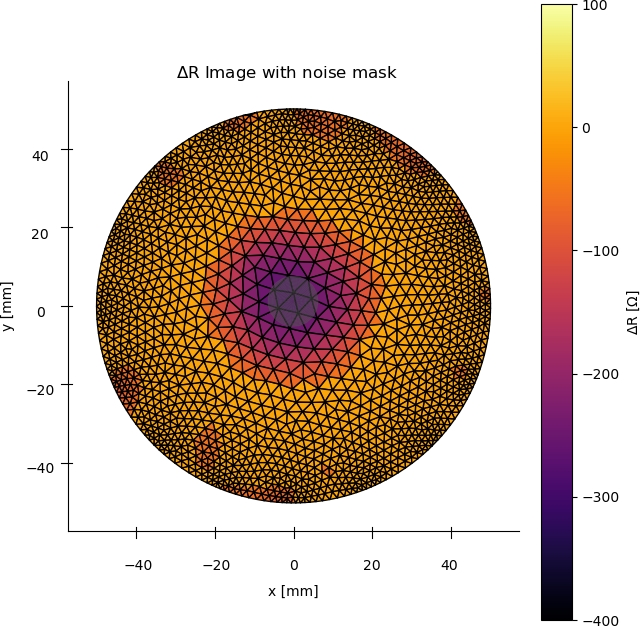
\includegraphics[width=0.6\linewidth]{Figures/CBSR_8p_9push_20strain_60s_4_frame20_noise_mask.jpg}
	\caption{Before executing the performance metrics calculations, the noise floor mask was applied to the 8\% CBSR material shown in Figure \ref{fig:CBSR sample and holder}}
	\label{fig:noise_floor_mask_8p}
\end{figure}


\section{More Threshold Percentage Masks}
\begin{figure}[H]
	\centering
	\begin{minipage}[t]{0.3\textwidth}
		\vspace{0pt}
		\subfloat[][]{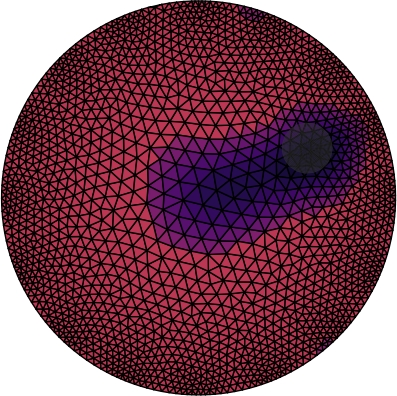
\includegraphics[width=\textwidth]{Figures/CBSR_9p_2_9push_25strain_60s_1mA_4_frame100_25p_mask_crop.jpg}\label{thresh25}}
		\vfill
		\subfloat[][]{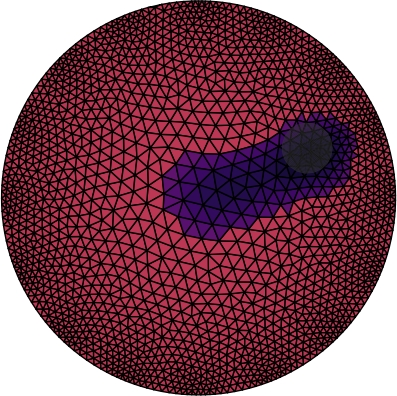
\includegraphics[width=\textwidth]{Figures/CBSR_9p_2_9push_25strain_60s_1mA_4_frame100_50p_mask_crop.jpg}\label{thresh50}}
		\vspace{0pt}
	\end{minipage}%
	\begin{minipage}[t]{0.3\textwidth}
		\vspace{0pt}
		\subfloat[][]{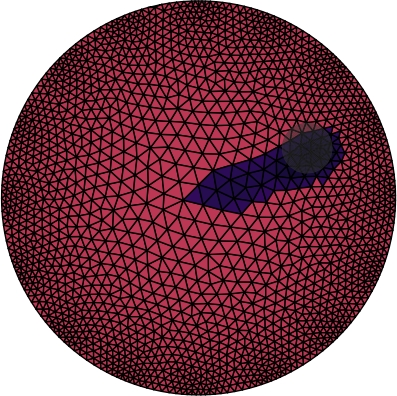
\includegraphics[width=\textwidth]{Figures/CBSR_9p_2_9push_25strain_60s_1mA_4_frame100_75p_mask_crop.jpg}\label{thresh75}}
		\vfill
		\subfloat[][]{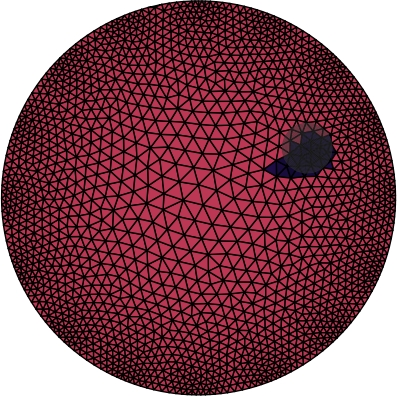
\includegraphics[width=\textwidth]{Figures/CBSR_9p_2_9push_25strain_60s_1mA_4_frame100_85p_mask_crop.jpg}\label{thresh85}}
		\hfill
	\end{minipage} 
	\begin{minipage}[t]{.1\textwidth}
		\vspace{0pt}
		\subfloat[][]{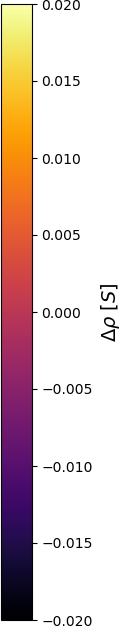
\includegraphics[width=\textwidth]{Figures/CBSR_9p_2_9push_25strain_60s_1mA_4_frame100_scale_bar.jpg}\label{colour_bar}}
		\hfill
	\end{minipage}  
	\caption{A series of threshold percentage masks (a) 25\%, (b) 50\%, (c) 75, and (d) 85\% for the same reconstruction given in Figure \ref{fig:noise_floor_mask_9p}. (e) is the resistance change scale bar.}
	\label{fig:thresh_masks}
\end{figure}

\section{Quasi-static Conductance Strain Fitted  Data}
\begin{figure}[H]
	\centering
	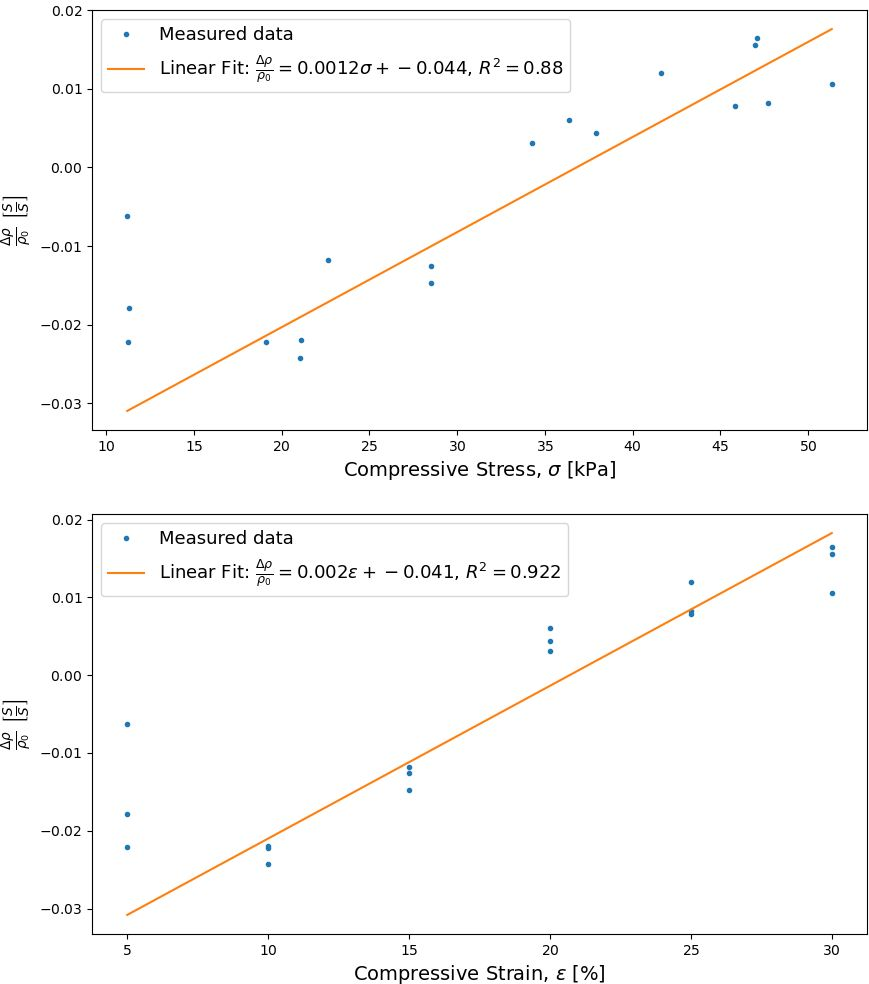
\includegraphics[width=0.7\linewidth]{Figures/CBSR_9p_cond_stress_strain_sin_titulo.jpg}
	\caption{Conductance change vs. stress (top) and strain (bottom) data and fitted curves for 9 wt\% CBSR. The 5\% strain values ignored as the $\mathrm{std}$ were larger than the conductance change values.}
	% TODO?: Change Linear fit to 10^{-1} from 10^{-3}
	\label{fig:quasi_r_9p}
\end{figure}

\section{1D and 2D Strain Settling Times}\label{apdx:Strain Relaxations}
\begin{figure}[H]
	\centering
	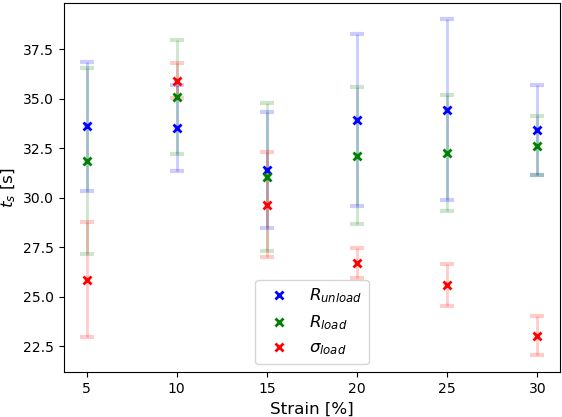
\includegraphics[width=0.8\linewidth]{Figures/CBSR_8p_1_10push_XXstrain_60s_ts_vals_vs_strain.jpg}
	\caption{Mean settling times for 5 - 30\% compressive strain applied to CBSR 8 wt\% with the error bars showing the standard deviation from 1D compressive test data.}
	\label{fig:strain_ts_8p_1D}
\end{figure}
\begin{figure}[H]
	\centering
	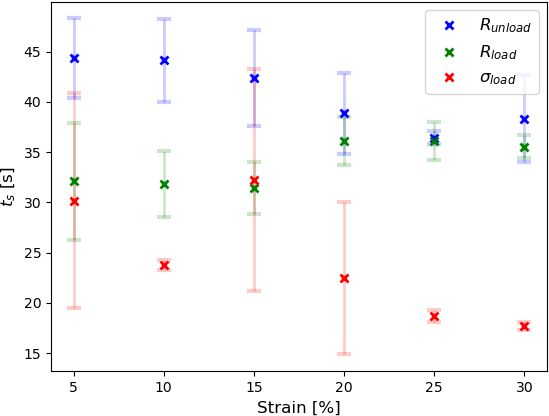
\includegraphics[width=0.8\linewidth]{Figures/CBSR_9p_1_3push_XXstrain_240s_ts_vals_vs_strain.jpg}
	\caption{Mean settling times for 5 - 30\% compressive strain applied to CBSR 9 wt\% with the error bars showing the standard deviation from 1D compressive test data.}
	\label{fig:strain_ts_9p_1D}
\end{figure}
\begin{figure}[H]
	\centering
	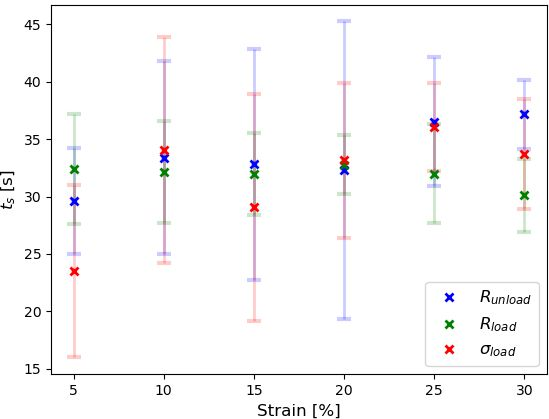
\includegraphics[width=0.8\linewidth]{Figures/CBSR_8p_1_9push_XXstrain_60s_X_ts_vals_vs_strain.jpg}
	\caption{Mean settling times for various strains applied to CBSR 8 wt\% with the error bars showing the standard deviation of each settling time from the 2D EIT experimental data.}
	\label{fig:strain_ts_8p}
\end{figure}
\begin{figure}[H]
	\centering
	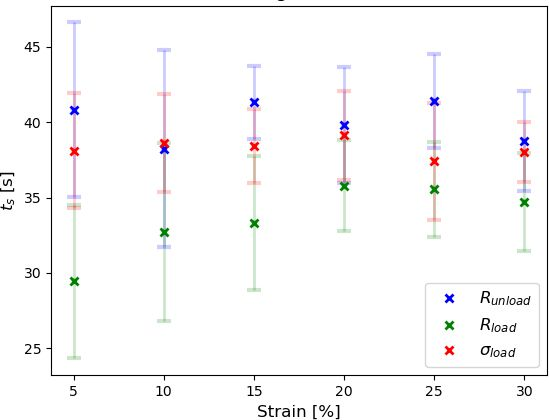
\includegraphics[width=0.8\linewidth]{Figures/CBSR_9p_2_9push_XXstrain_60s_1mA_X_ts_vals_vs_strain.jpg}
	\caption{Mean settling times for various strains applied to CBSR 9 wt\% with the error bars showing the standard deviation of each settling time from the 2D EIT experimental data.}
	\label{fig:strain_ts_9p}
\end{figure}


\section{Performance Metrics Example}\label{apdx:Performance Metrics}
\begin{figure}[H]
	\centering
	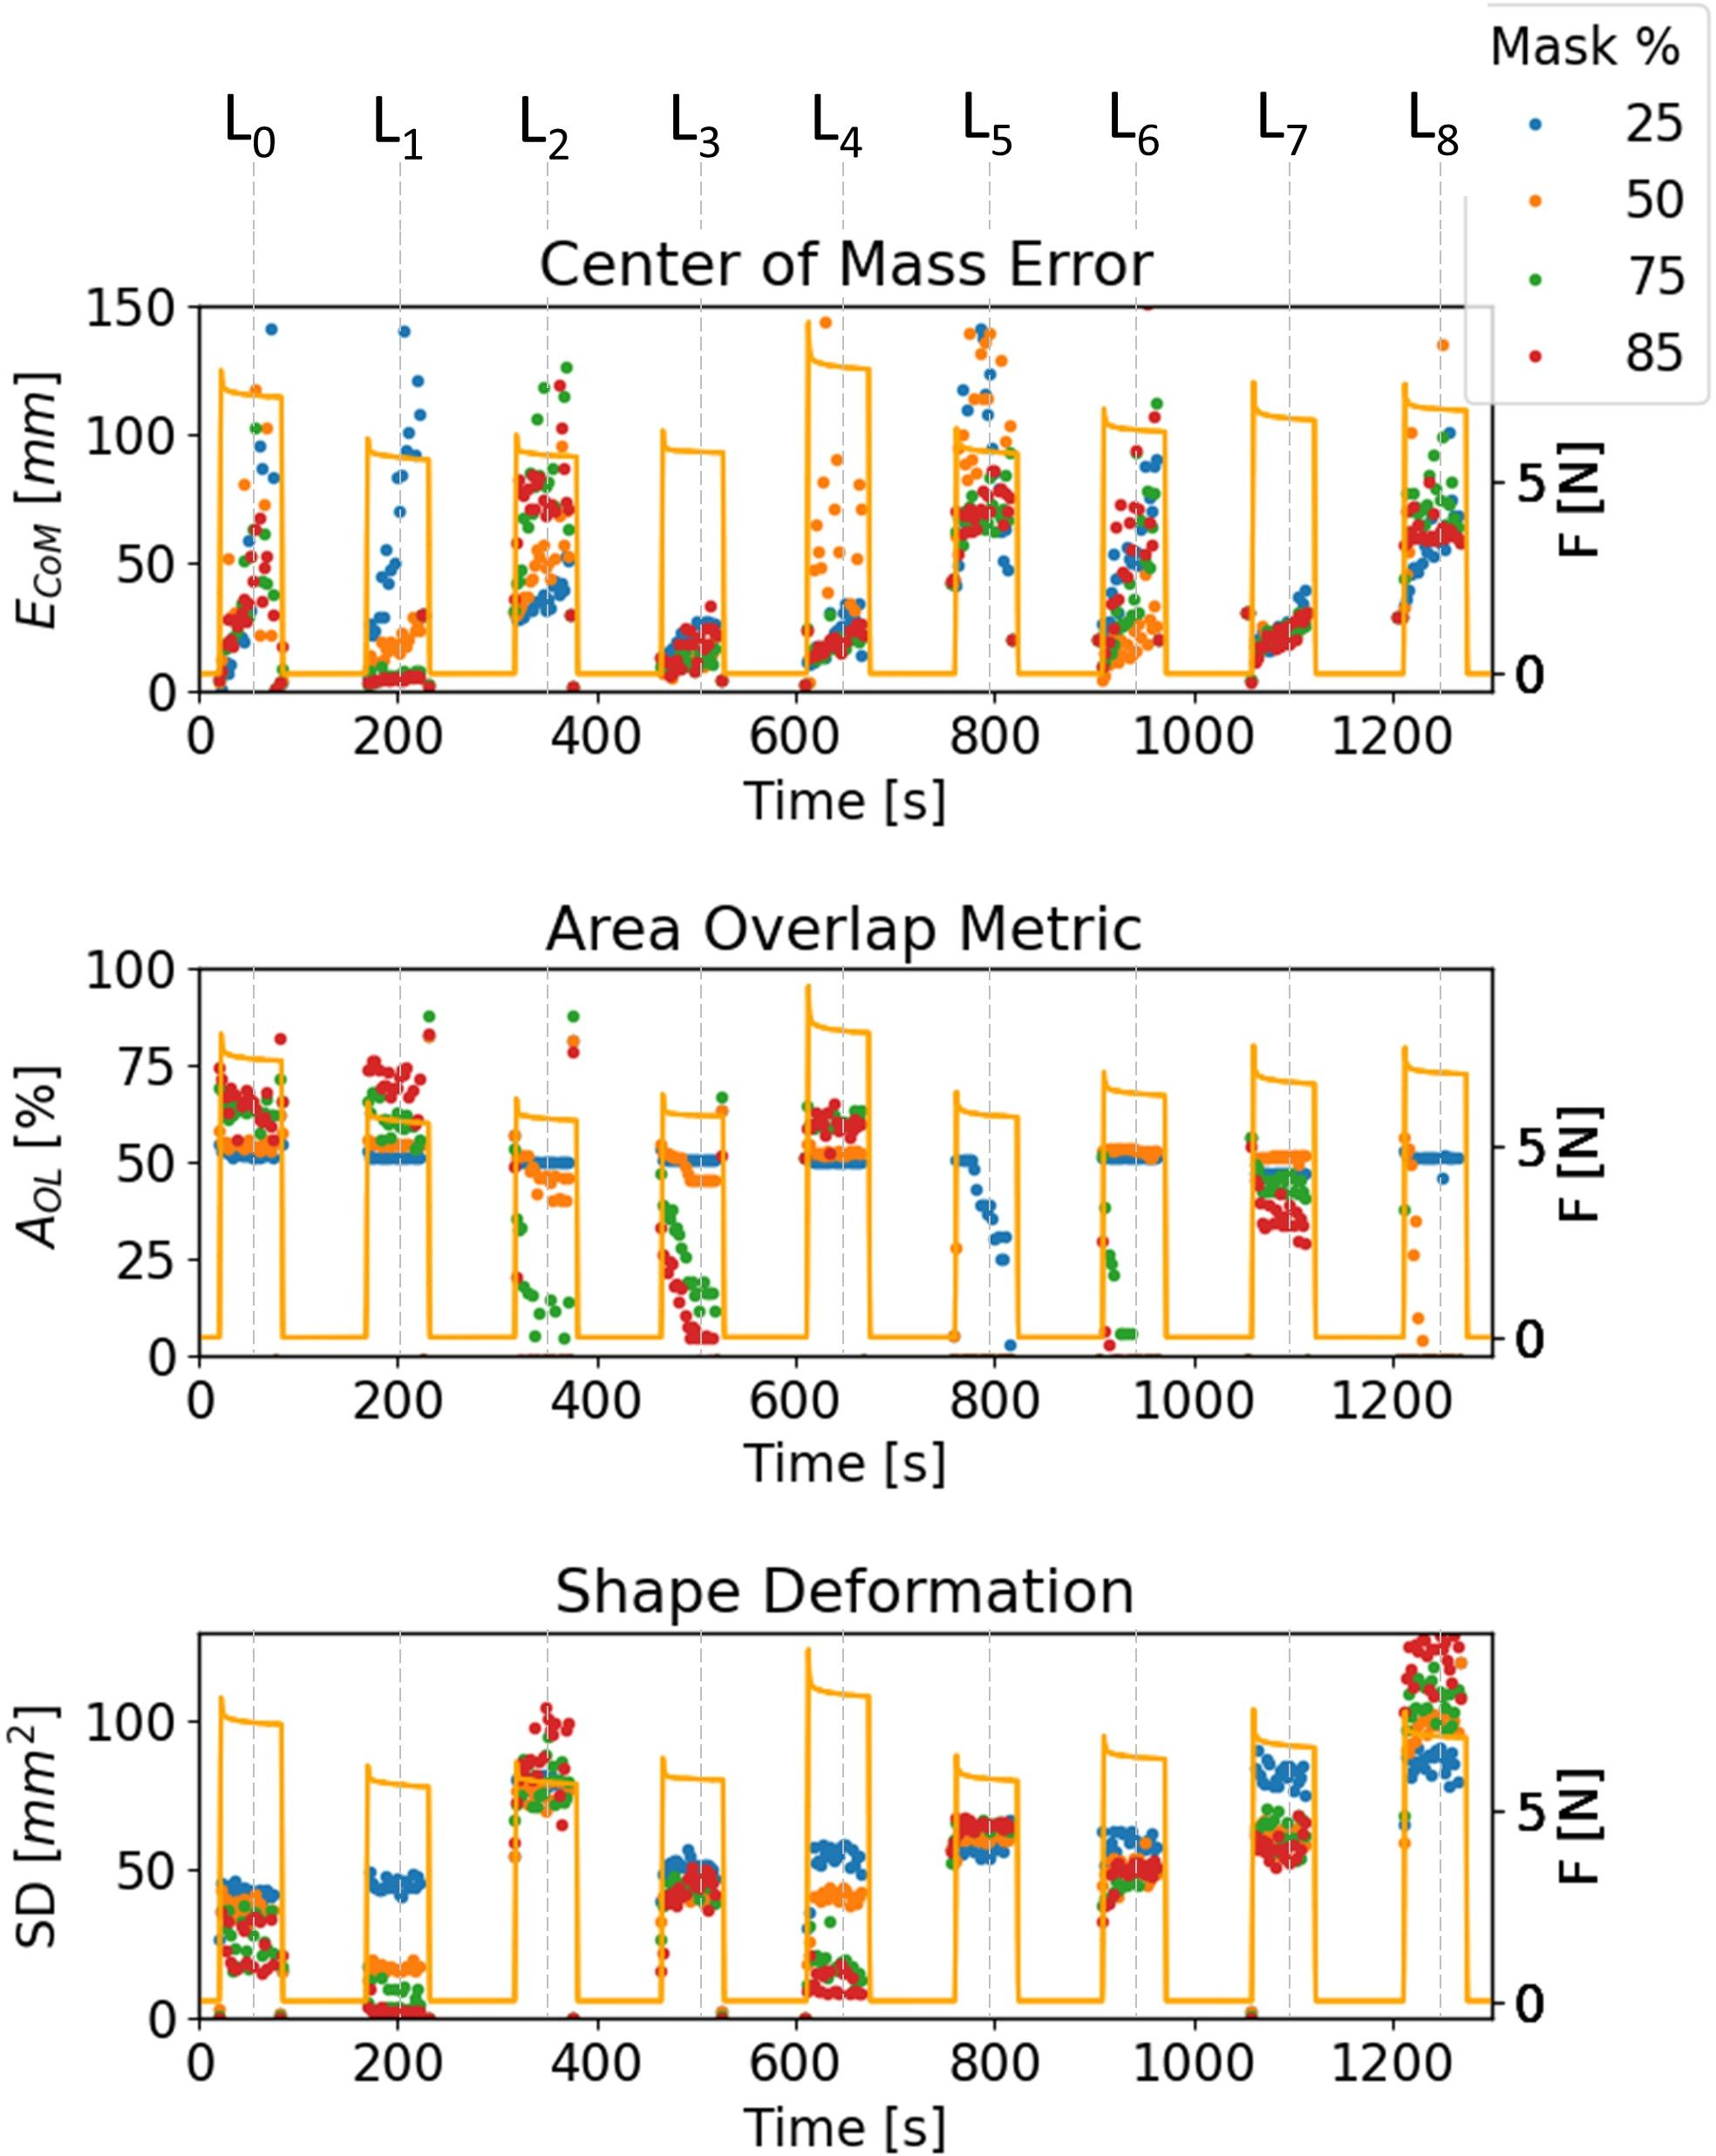
\includegraphics[width=0.8\linewidth]{Figures/CBSR_9p_9push_20strain_60s_4_metrics_thresh_masks_v2_numbd.jpg}
	\caption{Spatial performance metrics comparing threshold percentages of 25, 50, 75, and 85\% for 9 wt\% CBSR sample being loaded with 20\% compressive strain in nine areas, $L_{0-8}$, shown in Fig \ref{fig:force_app_map}.} % TODO?: Determine better way of displaying these metrics??
	\label{fig:recon_perform_9p}
\end{figure}

\section{Randomised test $S\!D$ metrics data}

\begin{table}[H]
	\caption{CBSR 8 and 9 wt\% mean and standard deviation for $S\!D$ spatial performance metrics of ten random locations, $L_{rand}$ and random strains $\varepsilon$}. % TODO: complete these tests with best blob algorithm??
	\label{tab:spatial_sd_metrics_stats_8p_rand_loads}
	\centering
	\hspace{0.4cm}
	\begin{tabular}{p{2.5cm}p{0.8cm}p{1.8cm}p{1.8cm}}
		\hline       
		$L_{rand}$(r, $\theta$) [mm, $\degree$] & $\varepsilon$ [\%] & 8wt\% $S\!D$ [mm] & 9wt\% $S\!D$ [mm] \\ \hline
		(5.4, 10) & 17.9 & 10.1 $\pm$ 0.8 & 9.8 $\pm$ 0.6\\
		(29.8, 337) & 24.0 & 62.2 $\pm$ 1.3 & 52.8 $\pm$ 1.3\\
		(4.2, 317) & 17.0 & 18.7 $\pm$ 5.9 & 21.7 $\pm$ 2.2\\
		(34.0, 70) & 10.9 & 20.2 $\pm$ 4.7 & 13.7 $\pm$ 0.8\\
		(35.8, 137) & 8.1 & 124.7 $\pm$ 2.8 & 81.5 $\pm$ 13.8\\
		(9.6, 55) & 13.8 & 24.8 $\pm$ 1.9 & 19.2 $\pm$ 1.8\\
		(2.8, 260) & 7.0 & 15.6 $\pm$ 4.5 & 12.7 $\pm$ 1.0\\
		(11.2, 114) & 10.0 & 4.5 $\pm$ 0.9 & 4.6 $\pm$ 0.6\\
		(24.6, 241) & 28.5 & 2.6 $\pm$ 0.1 & 2.6 $\pm$ 0.1\\
		(16.6, 253) & 23.6 & 0.3 $\pm$ 0.1 & 1.1 $\pm$ 0.1\\
		\hline
	\end{tabular}
\end{table}